\chapter{Accuracy of Monocular Tracking using Error Covariance Matrix}
\label{chap:Accuracy of Monocular Tracking using Error Covariance Matrix}

In \cite{bauer2007tracking}
an approach using error covariance matrix to represent the accuracy of monocular tracking is introduced. However this approach does not apply to our situation and I regard the method mentioned in this paper with suspicion. In this section I will explain in detail why this method does not work for our situation.

\section{Gaussian error distributions}

\subsection{Multi-dimensional Gaussian distributions}
\textbf{Gaussian distribution} is a very common continuous probability distribution. In our project we also set the image noisy(errors) as Gaussian distribution. We directly focus on the \textit{n}-dimensional Gaussian distribution which is shown in figure \ref{fig:gaussian}, the form of corresponding probability density function is:

\begin{align}\label{eq:cee1}
 f_{\mu,\Sigma}(x)= \frac{1}{\sqrt{( 2\pi)^n|\Sigma|}}exp^{\big(-\frac{1}{2}(x - \mu)^T \Sigma^{-1} (x - \mu) \big)}
\end{align}
where $\mu \in \mathbb{R}^n$ denotes the mean of random variable vector and $\Sigma \in \mathbb{R}^{n \times n}$ covariance matrix.

\begin{figure}[h!]
\centering
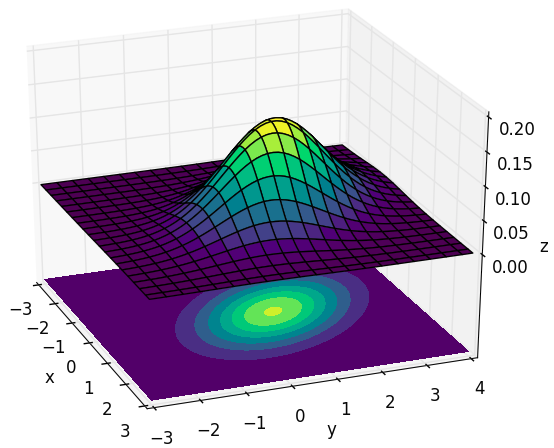
\includegraphics[scale=0.5]{./fig/gaussian.png}
\caption{Probability density function of 2 dimensional Gaussian distribution}  
\label{fig:gaussian}
\end{figure}

A \textit{n}-dimensional covariance matrix $\boldsymbol{\Sigma}$ is always symmetric and positive semi-definite, which means the eigenvalues of covariance matrix are non-negative.

\begin{align*}
\Sigma =   \begin{bmatrix} var(x1) & cov(x_1,x_2) & \cdots & cov(x_1,x_n) \\
                 cov(x_1,x_2) & var(x2) & \cdots & cov(x_n,x_2) \\
                 \vdots  & \vdots  & \ddots & \vdots  \\
                 cov(x_1,x_n) & cov(x_2,x_n) & \cdots & var(x_n) \\ \end{bmatrix} 
\end{align*}

\subsection{Confidence ellipse/ellipsoid}
The confidence ellipse which is also known as error ellipse represents an isocontour of the two dimensional Gaussian distribution and allow you to visualize the selected confidence level. In contrast to confidence ellipse, the confidence ellipsoid represents a visualization of three dimensional Gaussian distribution. 

Now we make a derivation from the probability function(equation \ref{eq:cee1}) and assume that the mean $\mu$ of random variable is zero:
\begin{align*}
p &= \frac{1}{\sqrt{( 2\pi)^n|\Sigma|}}exp^{\big(-\frac{1}{2}(x - \mu)^T \Sigma^{-1} (x - \mu) \big)}\\
\Downarrow \\
p \sqrt{( 2\pi)^n|\Sigma|} &= exp^{\big(-\frac{1}{2}(x - \mu)^T \Sigma^{-1} (x - \mu) \big)}\\
\Downarrow \\
(x - \mu)^T \Sigma^{-1} (x - \mu) &= -2 \ln{p \sqrt{( 2\pi)^n|\Sigma|}}\\
\Downarrow \\
x^T \Sigma^{-1} x &= -2 \ln{p \sqrt{( 2\pi)^n|\Sigma|}} = s
\end{align*}

In general, we can use following equations to describe ellipse and ellipsoid:

\begin{align*}
(\frac{x}{a})^2 + (\frac{y}{b})^2 &= 1 & \text{a,b: length of semi-major axis and length of semi-minor axis}\\
(\frac{x}{a})^2 + (\frac{y}{b})^2 + (\frac{z}{c})^2 &= 1 & \text{a,b,c: semi-axes}
\end{align*}

From covariance matrix we can derive the forms similar to the above equations:

\begin{align*}
\frac{x^2}{\lambda_x} + \frac{y^2}{\lambda_y} &= s \\
\frac{x^2}{\lambda_x} + \frac{y^2}{\lambda_y} + \frac{z^2}{\lambda_z} &= s
\end{align*}
where $\lambda_x$, $\lambda_y$ and $\lambda_z$ are the eigenvalues of the corresponding covariance matrix, \textit{s} defines the scale of the ellipse which could be any arbitrary number. Then we turn the question into how to find \textit{s}, in our case we use confidence level to represent the scale \textit{s}. The relationship between confidence level and scale \textit{s} for different dimensions is shown in table \ref{table:confidence_level}.

\begin{table}[h]
\begin{tabular}{ |l|l|l|l|l|l|l| }
\hline
\multicolumn{7}{ |c| }{Confidence Level} \\
\hline
Dimension & 25\% & 50\% & 75\% & 95\% & 97\% & 99\% \\ \hline
n = 1 & 0.10153  & 0.45494 & 1.3233 & 3.84146 & 4.70929 &  6.6349\\
n = 2 & 0.57536  & 1.38629 & 2.77259 & 5.99146 & 7.01312 &  9.2103 \\
n = 3 & 1.21253  & 2.36597 & 4.10834 & 7.81473 & 8.94729 &  11.3449 \\
\hline
\end{tabular}
\caption[Table caption text]{The value of scale \textit{s} in different confidence levels for different dimensions. e.g. if n = 2 and confidence level is 95\% then the scale \textit{s} is 5.99146\cite{bauer2007tracking}}
\label{table:confidence_level}
\end{table}

Now we make a transform of ellipse and ellipsoid, multiply $\frac{1}{s}$ on both sides of equations:
\begin{align*}
(\frac{x}{ \sqrt{s\lambda_x}})^2 + (\frac{y}{\sqrt{s\lambda_y }})^2 &= 1 \\
(\frac{x}{\sqrt{s\lambda_x }})^2 + (\frac{y}{\sqrt{s\lambda_y }})^2 + (\frac{z}{\sqrt{s\lambda_z }})^2 &= 1
\end{align*}

we find that the length of the axes of ellipse or ellipsoid can be represented as $l_i = \sqrt{s\lambda_i}(i = 1,2,3)$. We can use this formula to calculate the length of axes and then plot the covariance ellipse or ellipsoid for a certain confidence level as an example shown in figure \ref{fig:confidence2D} and figure \ref{fig:ellipsoid}.

\begin{figure}[h!]
\centering
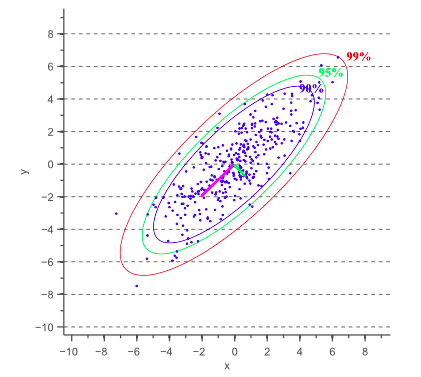
\includegraphics[width=0.9\textwidth]{./fig/confidence2D.png}
\caption{Confidence ellipses for normally distributed data with different confidence levels\cite{vincent_spruyt}} 
\label{fig:confidence2D}
\end{figure}


\begin{figure}[h!]
\centering
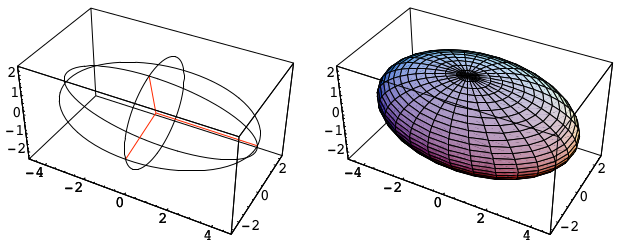
\includegraphics[width=0.9\textwidth]{./fig/ellipsoid.png}
    \caption{Visualization of covariance ellipsoid for a certain confidence level\cite{bauer2007tracking}}
\label{fig:ellipsoid}
\end{figure}

\section{Error propagation for Gaussian distributions} 
Two propagation methods are introduced in ...%
which are used to describe Gaussian errors propagation in linear or non-linear functions of monocular tracking system.
\section{Forward propagation} 
For the linear function, if the random variable $\textit{v}$ is a Gaussian distribution then the linear function $f(v)$ is also a Gaussian distribution. We assume that the linear function is describe as $f(v) = Av$, the mean of variable $\textit{v}$ is $\overline{v}$ and the covariance matrix is $\Sigma$. Then the linear function $f(v)$ is also a random variable with mean $f(\overline{v})$ and covariance matrix $\Sigma_f$. This relationship is shown in table \ref{table:linear_function}:

\begin{table}[h!]
\begin{center}
\begin{tabular}{ |l|l|l| }
\hline
 & mean & covariance matrix \\ \hline
$v$ & $\overline{v}$  & $\Sigma$ \\
$f(v)$ & $f(\overline{v})$ & $\Sigma_f = A \Sigma A^T$ \\
\hline
\end{tabular}
\caption[Table caption text]{Linear function: $f(v) = Av $}
\label{table:linear_function}
\end{center}
\end{table}

For the non-linear function $f(v)$, in order to apply the Gaussian distribution forward propagation we need to build an approximation of the non-linear function. We can use Taylor expansion to  present the first order approximation:

\begin{align*}
f(v) = f(v_0 + \Delta_v) = f(v_0) + J_f(v_0)\Delta_v + \mathcal{O}{v^2}
\end{align*}

For the non-linear function $f(v)$ we assume that the mean of variable $\textit{v}$ is $\overline{v}$ and the covariance matrix is $\Sigma$. Then the non-linear function $f(v)$ is a random variable with mean $f(\overline{v})$ and covariance matrix $\Sigma_f$. This relationship is shown in table \ref{table:nonlinear_function}:

\begin{table}[h!]
\begin{center}
\begin{tabular}{ |l|l|l| }
\hline
 & mean & covariance matrix \\ \hline
$v$ & $\overline{v}$  & $\Sigma$ \\
$f(v)$ & $f(\overline{v})$ & $\Sigma_f = J_f \Sigma J_f^T$ \\
\hline
\end{tabular}
\caption[Table caption text]{Non-linear function: $f(v)$}
\label{table:nonlinear_function}
\end{center}
\end{table}

where $J_f$ is the Jacobian matrix of non-linear function $f(v)$ evaluated at $\overline{v}$.

\section{Backward propagation} 

In some situation if the covariance matrix $\Sigma_f$ of function $f(v)$ is given and we want to know the covariance $\Sigma$ of the variable \textit{v}. We can use the following equation to compute the backward propagation:

\begin{align*}
\Sigma = (J_f^T \Sigma_f^{-1} J_f)^{-1}
\end{align*}

where $J_f$ is the Jacobian matrix of non-linear function $f(v)$ evaluated at $\overline{v}$.
This backward propagation is the main idea to compute the accuracy of monocular tracing in \cite{bauer2007tracking}

\section{Accuracy of monocular tracking}
In \cite{bauer2007tracking}
the computation of accuracy of monocular tracking is under a theoretical model, which the topology of the target is known exactly and all the features from the target can be well recognized and that the 2D position estimation is unbiased but not noise free. In \cite{bauer2007tracking}
a spherical coordinate system is used to represent the pose of camera in world.

\begin{figure}[h!]
\centering
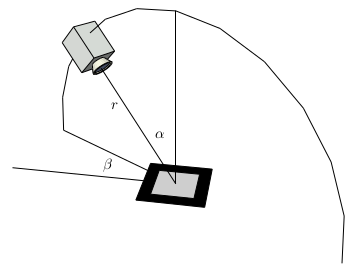
\includegraphics[width=0.5\textwidth]{./fig/spherical.png}
    \caption{Setup for analyzing the theoretical accuracy of a monocular tracking
system with planar fiducials\cite{bauer2007tracking}}
\label{fig:spherical}
\end{figure}

In this case the camera pose can be described with 3 parameters($\alpha,\beta,r$) instead of six-dimensional pose($x,y,z,\alpha,\beta,\gamma$), so a covariance matrix $\Sigma_{\alpha,\beta,r} \in \mathbb{R}^{n \times n}$ can represent the error for each camera position.

Recall that the pinhole camera model, the relationship between world coordinate system and pixel coordinate system.
\begin{equation}\label{eq:zckt}
Z_C \begin{bmatrix} u \\ v \\ 1 \end{bmatrix}
      = KT                                         
        \begin{bmatrix} X_W \\ Y_W \\ Z_W \\ 1 \end{bmatrix}                 
\end{equation}
where camera intrinsic parameters \textbf{K} is constant and in our situation we set it as:
\begin{equation*}
K =  \begin{bmatrix} 800 & 0 & 320 \\ 0 & 800 & 240 \\ 0 & 0 & 1\end{bmatrix}                 
\end{equation*}
According to \cite{bauer2007tracking}
without loss of generality the camera extrinsic parameters \textbf{T}([\textbf{R}$|$\textbf{t}]) can be parametrized with $\alpha,\beta,\gamma$ and the following equations show how to get the rotation matrix \textbf{R} based on coordinate transformation, this process is shown in figure \ref{fig:NAB}.
\begin{align*}\label{eq:nrb}
\tensor*[^N]{R}{^B} &= \tensor*[^N]{R}{^A} \cdot \tensor*[^A]{R}{^B}\\
               &=\begin{bmatrix} 
                cos(\alpha)cos(\beta) & -sin(\beta) & sin(\alpha)cos(\beta) \\
                cos(\alpha)sin(\beta) & cos(\beta) & sin(\alpha)sin(\beta)  \\
                sin(\alpha) & 0 & cos(\alpha)
                \end{bmatrix} 
\end{align*}
Because the positive direction of the camera \textit{z}-axis always points to the origin where the marker is placed in the world coordinate system, the rotation matrix $\tensor*[^N]{R}{^B}$ still needs to rotate $\SI{180}{\degree}$ around \textit{x}-axis:
\begin{align*}
R = R_x(\pi) \cdot \tensor*[^N]{R}{^B}\\
\end{align*}

\begin{figure}[h!]
\centering
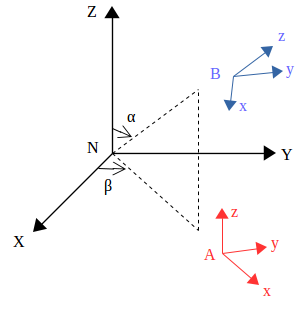
\includegraphics[width=0.5\textwidth]{./fig/NAB.png}
    \caption{Rotation in spherical coordinate system}
\label{fig:NAB}
\end{figure}

And from Cartesian coordinates to spherical coordinates transformation we know that the translation vector \textbf{t} can be presented using there parameters $\alpha,\beta,\gamma$ as:
\begin{align*}
x &= r \cdot cos(\beta) \cdot sin(\alpha) \\
y &= r \cdot sin(\beta) \cdot sin(\alpha)\\
z &= r \cdot cos(\alpha)
\end{align*}
Now the camera extrinsic parameters \textbf{T}([\textbf{R}$|$\textbf{t}]) can be presented as:
\begin{align*}
T &=\begin{bmatrix} 
                cos(\alpha)cos(\beta) & -sin(\beta) & sin(\alpha)cos(\beta) & r cos(\beta) sin(\alpha)\\
                cos(\alpha)sin(\beta) & cos(\beta) & sin(\alpha)sin(\beta)  & r sin(\beta) sin(\alpha)\\
                sin(\alpha) & 0 & cos(\alpha) & r cos(\alpha) \\
                0 & 0 & 0 & 1                
                \end{bmatrix} 
\end{align*}
Because we already know the expression of the camera extrinsic parameters \textbf{T} with $\alpha,\beta,\gamma$ and the camera intrinsic parameters \textbf{K} is constant, now we can split the equation \ref{eq:zckt} into two parts:
\begin{equation}\label{eq:fjacobian}
 f(\alpha,\beta,r) : 
  \begin{cases} 
     u := A_1 \alpha + B_1 \beta + C_1 r \\
     v := A_2 \alpha + B_2 \beta + C_2 r 
  \end{cases}
\end{equation}
where $\mathit{A_1,B_1,C_1,A_2,B_2,C_2}$ are the coefficients come from \textbf{KT}. Sequentially we can compute the \textit{Jacobian} of function \ref{eq:fjacobian} evaluated at the origin:
\begin{align}\label{eq:evaluated}
J_f =  
\left.\frac{\partial f}{\partial(\alpha,\beta,r)}\right|_0 \in \mathbb{R}^{2n \times 3}
\end{align} 
where \textit{n} is the number of image points(we set $n = 4$ in our simulation).\\
In our case we set image noises as 2-dimensional Gaussian distribution, so the error for each image point can be detected with uncertainty given by the covariance matrices $\Sigma_{v_i} \in \mathbb{R}^{2 \times 2}$. And reference the \textbf{backward propagation} theory the covariance matrix for detecting the planar marker can be represented as:                
\begin{align*}
\Sigma_{\alpha,\beta,r} = \begin{pmatrix}
 J_f^T 
                \begin{bmatrix} 
                  \Sigma_{v1} & \quad & \quad\\ 
                  \quad & \ddots & \quad \\
                  \quad & \quad & \Sigma_{vn}
                \end{bmatrix}^{-1} 
 J_f
                          \end{pmatrix}^{-1}
                          \in \mathbb{R}^{3 \times 3}
\end{align*}
From equation \ref{eq:evaluated} the \textit{Jacobian} of \textit{f} is evaluated at the origin($\alpha = 0,\beta = 0,\gamma = 0$), which means $J_f$ is always a constant matrix no matter where the image point is. If the value of $\mathbf{J_f}$ is constant, this leads to a big problem: \textbf{The value of} ${\Sigma_{\alpha,\beta,r}}$  \textbf{only depends on the set of covariance matrices} $                \begin{bmatrix} 
                  \Sigma_{v1} & \quad & \quad\\ 
                  \quad & \ddots & \quad \\
                  \quad & \quad & \Sigma_{vn}
                \end{bmatrix}^{-1}$. 
And image noise of each point is set as 2-dimensional Gaussian distribution with the mean 0 and standard deviation 2. So the diagonal terms of the covariance matrix $\Sigma_{v_i}$ of each image points with error are closed to 4(it depends on the size of samples) and the rest terms of $\Sigma_{v_i}$ are closed to 0. So we get the following approximate value when n = 4:
\begin{align*}
                \begin{bmatrix} 
                  \Sigma_{v1} & \quad & \quad & \quad\\ 
                  \quad & \Sigma_{v2} & \quad & \quad\\ 
                  \quad & \quad & \Sigma_{v3} & \quad\\ 
                  \quad & \quad & \quad & \Sigma_{v4}\\ 
                \end{bmatrix}^{-1} 
                \approx
                \begin{bmatrix} 
                  2 & 0 & 0 & 0 & 0 & 0 & 0 & 0 \\
                  0 & 2 & 0 & 0 & 0 & 0 & 0 & 0 \\
                  0 & 0 & 2 & 0 & 0 & 0 & 0 & 0 \\
                  0 & 0 & 0 & 2 & 0 & 0 & 0 & 0 \\
                  0 & 0 & 0 & 0 & 2 & 0 & 0 & 0 \\
                  0 & 0 & 0 & 0 & 0 & 2 & 0 & 0 \\
                  0 & 0 & 0 & 0 & 0 & 0 & 2 & 0 \\
                  0 & 0 & 0 & 0 & 0 & 0 & 0 & 2 \\                  
                \end{bmatrix}^{-1} 
\end{align*}

We can easily find that the diagonal terms of the covariance matrix $\Sigma_{v_i}$ play a decisive role in backward propagation formula. Based on these almost similar $\Sigma_{v_i}$ the covariance matrix $\Sigma_{\alpha,\beta,r}$ of different image points only has a extremely tiny change, \textbf{the value of} $\Sigma_{\alpha,\beta,r}$ \textbf{can be almost regarded as constant}! 

According to the above explanation we can not display covariance ellipsoids exactly like figure \ref{fig:cov_ellip}. From this view the accuracy of monocular tracking method introduced in \cite{bauer2007tracking}
can not be applied to our situation! Whether this method can be applied to other situations, I am still skeptical about this.

\begin{figure}[h!]
\centering
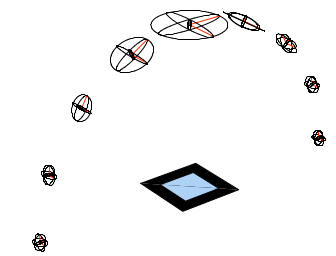
\includegraphics[width=0.5\textwidth]{./fig/cov_ellip.png}
    \caption{Accuracy of the pose of the camera in marker coordinates. Display with covariance ellipsoids\cite{bauer2007tracking}}
\label{fig:cov_ellip}
\end{figure}
